\chapter{本研究における問題定義と仮説}
\label{appr}

本章では,~\ref{intr}章で述べた背景より,本章では,現状のHoneypotの問題点を整理し,この問題をどのように解決すれば良いのかを定義する.

\section{本研究における問題定義}
\label{appr:problem}
現状のHoneypotの問題点を列挙していき,整理する.

\subsection{SSH\,Honeypotの現状の問題}
\label{appr:problemofSshHoneypot}
Honeypotには運用する上で大きな問題が2つある.一つは設置したHoneypotに侵入した悪意のある侵入者が侵入先をHoneypotであると検知してしまう問題である.もう一つはHoneypotに侵入を許した侵入者にHoneypotを設置した機器から攻撃が仕掛けられてしまう危険がある問題である.\\
以下の図2は,悪意のある侵入者が不正に機器に侵入してから踏み台にして他の機器に攻撃を仕掛けるまでの一般的なフロ--であるが,2番目のフロ--の悪意のある侵入者が侵入した先がHoneypotであると検知してしまうことや,高対話型Honeypotで使用したOS自体の新たな脆弱性を突かれることに限った状況では,3番目のフロ--のHoneypotに侵入を許した侵入者にHoneypotを設置した機器から攻撃が仕掛けられてしまう危険があることが今回の問題である.

\vspace{10mm}
\begin{figure}[H]
    \centering
    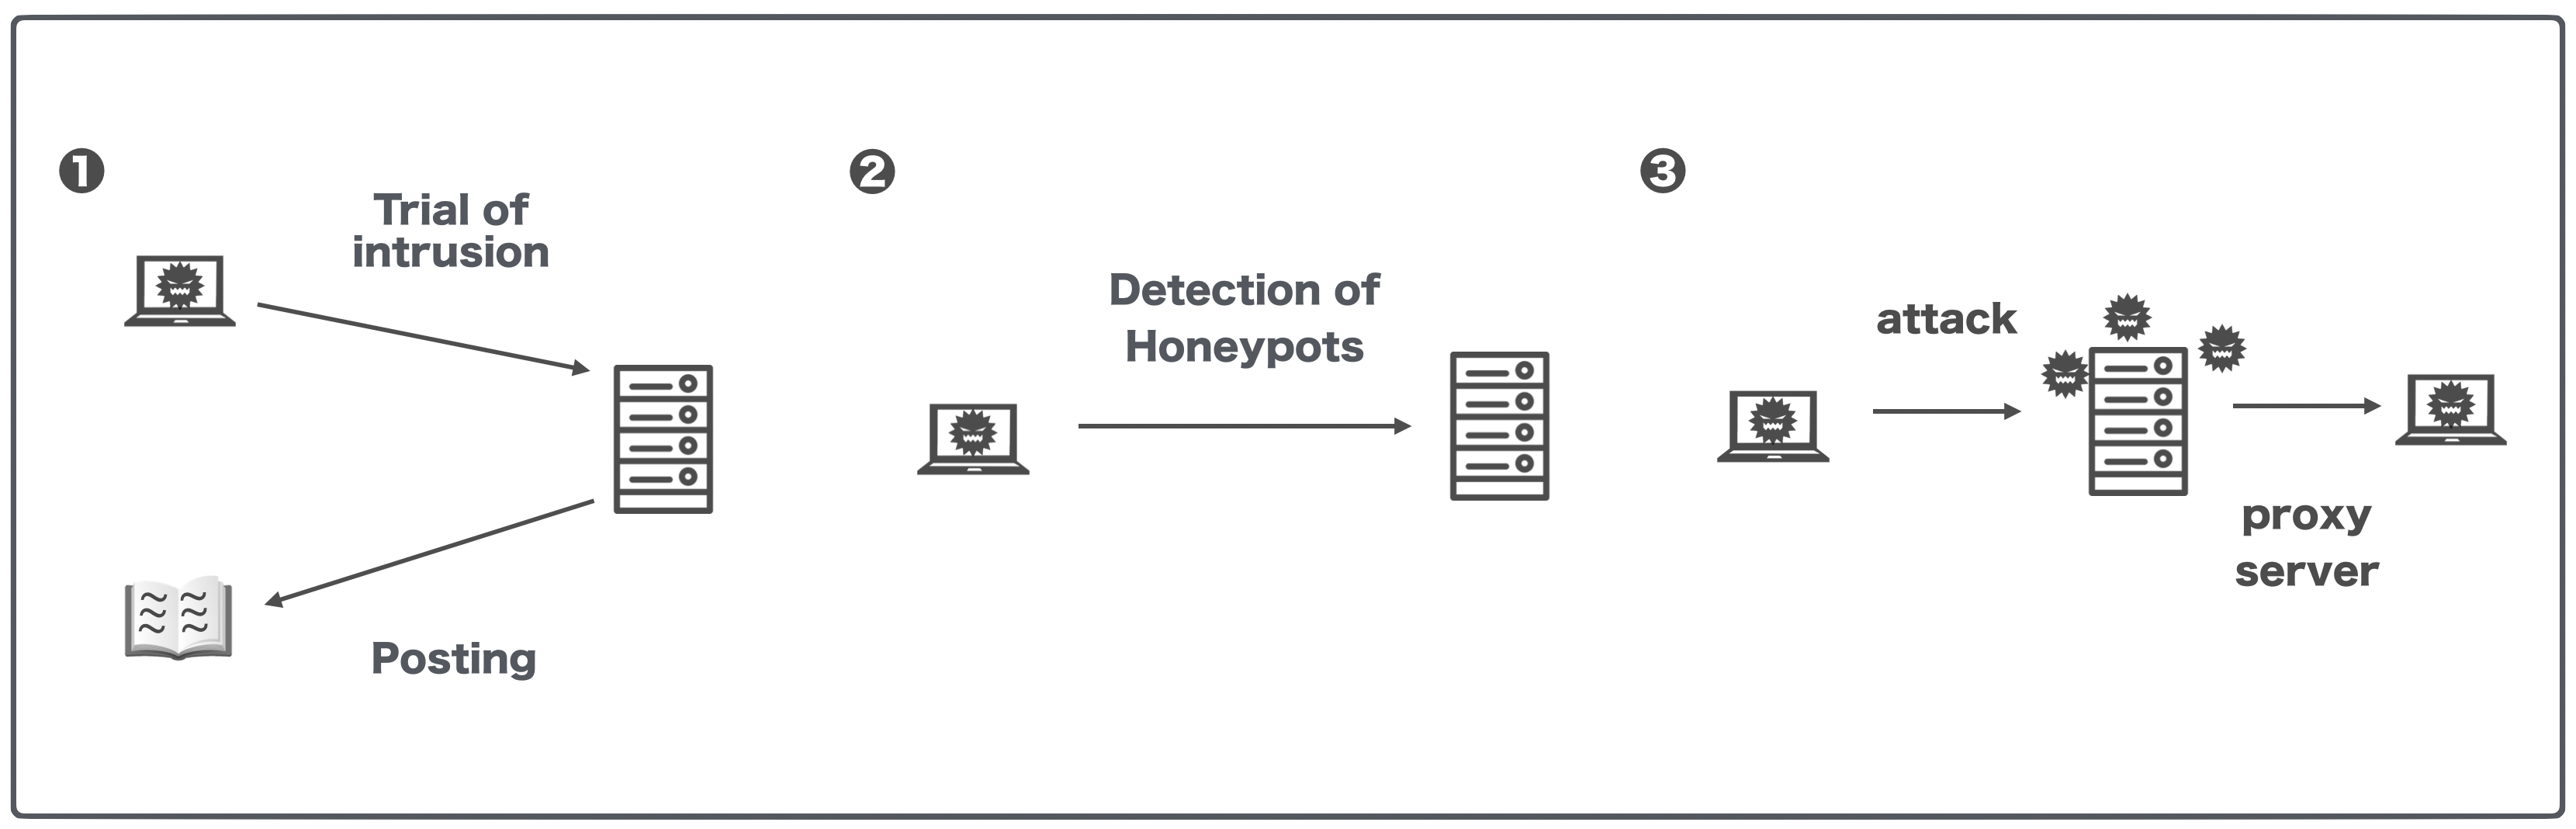
\includegraphics[width=1.0\textwidth]{figures/nagare.png}
    \caption{不正なSSH侵入者の想定行動フロー}
    \label{fig:evo}
\end{figure}

本研究ではこの中でも,2番目のフロ--のSSHの低対話型Honeypotが設置したHoneypotに悪意のある侵入者が侵入先をHoneypotであると検知してしまう問題に着目した.

\subsubsection{SSHの低対話型Honeypotにおける問題}
\label{appr:problemofSshLowHoneypot}
SSHの低対話型Honeypotは実際のShellの挙動をエミュレートしたものであるのでコマンドやその挙動についての機能が限定されており,実際のShellの機能として不足がある.またSSHの低対話型Honeypot特有の以上な挙動も存在する.さらに,SSHでHoneypotにセッションを確立する際に,そのレイテンシを計測し,そのレイテンシがHoneypotの場合に通常とは明らかに異なることにより,Honeypotであると検知されてしまう問題がある.また,Honeypotのusernameが"Richard"がデフォルトのため,usernameからHoneypotであることを検知されてしまう問題もある.これらの検知手法を用いて,侵入者に侵入先がHoneypotであると検知され,本来取れるはずの攻撃ログが収集できない問題がある.

\subsubsubsection{SSHでのセッション確立におけるレイテンシの問題}
\label{appr:LowHoneypotLatency}

\subsubsubsection{HoneypotのUsernameの問題}
\label{appr:LowHoneypotUsername}

\subsubsubsection{Honeypotのコマンドの実装の問題}
\label{appr:LowHoneypotCommand}
SSHの低対話型Honeypotは実際のShellの挙動をエミュレートしたものであるのでコマンドやその挙動についての機能が限定されており,実際のShellの機能として不足がある.~\ref{tech:BusyBox}で述べたように,"Linux上で最小の実行ファイル"となるよう設計されているBusyBoxに含まれるコマンドの数が200以上あるのに対し,現状で広く使われているSSHの低対話型HoneypotであるCowrieに実装されているコマンドは~\ref{tech:Cowrie}でも述べた通り,38しか存在しない.また,SSHの低対話型Honeypot特有の挙動が存在し,以下にその1例であるプログラム\,1とプログラム\,2を示す.

\vspace{5mm}
\lstnewenvironment{mylisting}[1][]
    {\lstset{
        frame=single,
        basicstyle=\ttfamily,
        numbers=left,
        numbersep=10pt,
        tabsize=2,
        extendedchars=true,
        xleftmargin=17pt,
        framexleftmargin=17pt,
        #1
    }
}{}

\begin{mylisting}[language=sh,caption=正しいShellの挙動]
nadechin@cpu:~$ echo -n test
testnadechin@cpu:~$
\end{mylisting}

\begin{mylisting}[language=sh,caption=Kippo特有の異常な挙動の例]
s15445ys@s15445ys-neco:~$ echo -n hello
-n hello
s15445ys@s15445ys-neco:~$
\end{mylisting}

プログラム\,3.1が通常の挙動でプログラム\,3.2がSSHの低対話型Honeypotの挙動である.echoコマンドの-nオプションは改行をしないようにするというものであるが,実際のShellの挙動が改行がされず,正しく出力されているのに対して,Honeypotの挙動ではオプション部分も出力されてしまう.これはSSHの低対話型Honeypot特有の挙動であるため,これによってHoneypotであると検知されてしまう可能性がある.

%\subsubsection{SSHの高対話型Honeypotにおける問題}
%\label{appr:problemofSshHighHoneypot}
%一方で高対話型Honeypotは,実際に脆弱性を残した実際のOSやアプリケーションシステムを利用したものであるので,侵入を許すと設置したOSの予期せぬ脆弱性を突かれたり新たなウイルスによってroot権限を取られ,設置したOSから他のホストへと攻撃してしまう可能性を含んでいるため,設置コストやリスクに問題がある.

\subsection{本研究の問題}
\label{appr:subproblem}
~\ref{appr:problemofSshLowHoneypot}で列挙したSSHの低対話型Honeypotの問題の中で,実際のShellに実装されているコマンドの不足がある.またSSHの低対話型Honeypotに特有の異常な挙動も存在するため,設置したHoneypotが悪意のある侵入者に侵入先をHoneypotであると検知されてしまい,実際のOSに悪意のある侵入者が侵入した時の侵入ログとの違いが大きく出てしまう問題に着目した.

\section{問題解決のための要点}
\label{appr:YotenForProblem}
~\ref{appr:subproblem}で着目した問題を解決するためには,以下2つの手法を取る必要がある.

\begin{itemize}
\setlength{\leftskip}{3.2cm}
 \item[コマンドの追加実装:] 実際のShellに実装されているコマンドで,SSHの低対話型Honeypotに実装されていないコマンドを実装する
 \item[既実装コマンドの修正:] SSHの低対話型Honeypotに特有の異常な挙動をする既実装コマンドを修正する
\end{itemize}


\section{仮説}
\label{appr:Hypothesis}
~\ref{appr:addcommand}と~\ref{appr:repaircommand}で示す問題解決のための要点を踏まえると,SSHの低対話型Honeypotに侵入した悪意のある侵入者に侵入先をHoneypotであると検知させず,SSHの低対話型Honeypotに悪意のある侵入者が侵入した時の侵入ログを,実際のOSに悪意のある侵入者が侵入した時の侵入ログに近似できるのでないかと考えた.

\subsection{コマンドの追加実装}
\label{appr:addcommand}
実際のShellに実装されているコマンドで,SSHの低対話型Honeypotに実装されていないコマンドを実装することで,Honeypotへの侵入者が実行できるコマンドの少なさによる,Honeypotであることの検知を回避することができる.

\subsection{既実装コマンドの修正}
\label{appr:repaircommand}
SSHの低対話型Honeypotに特有の異常な挙動をする既実装コマンドを修正することで,Honeypotについて認知している侵入者が,侵入先をHoneypotであると検知することを回避することができる.


%%% Local Variables:
%%% mode: japanese-latex
%%% TeX-master: "./thesis"
%%% End:
